\section{Music notation anatomy}

\subsection{Note names}

You have already seen the music staff from \ref{fig:music_note_names_on_staff} in the previous exercises. However, the meaning of it was not explained yet.

The letters A-G on the staff show which line on the staff has which note value. The notes that are in between the lines nicely spell out "FACE", making it easy to remember. The Note that are on the lines can be remembered with the mnemonic "\textbf{E}very \textbf{G}ood \textbf{B}oy \textbf{D}oes \textbf{F}ine". But another important thing to see is that the notes go up alphabetically (starting again with A after G). 

The most left symbol (\clefG) is called the G clef. Note that the curl of the G clef is on the line of the G note. 

The vertical line in the middle indicates the start/end of a new measure. and the thinner vertical line in at the end indicates the end of the piece.

\begin{figure}[h]
	\centering
	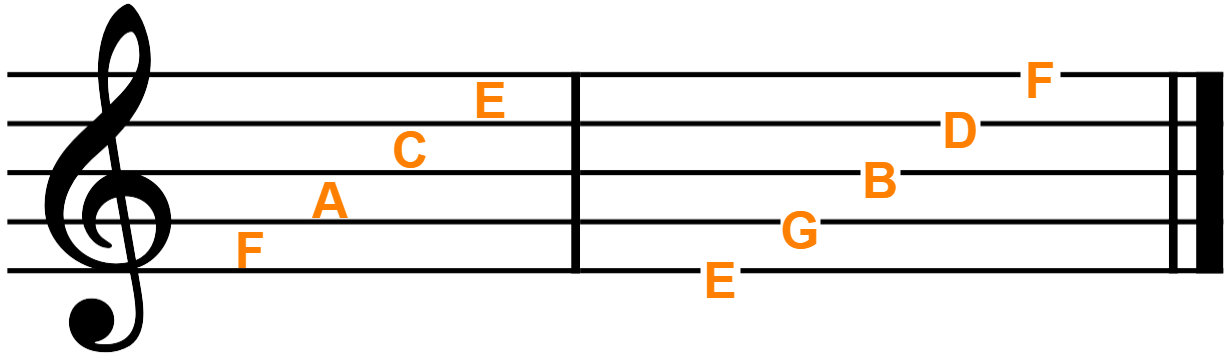
\includegraphics[width=0.6\textwidth]{../../Images/MusicNotation_MeasureNoteNames.png}
	\caption{Note names on the staff in two measures}
	\label{fig:music_note_names_on_staff}
\end{figure}

Note that the clef shown in \ref{fig:music_note_names_on_staff} is different than the ones seen in earlier exercises. For guitar notation you sometimes see a little 8 under de clef. This means that the original position of "middle C" (C4) with treble clef sounds an octave lower. This Results in the C that you see in \ref{fig:music_note_names_on_staff} to be the middle C (C4) when there is a little 8 below the clef.

\newpage

\subsection{Time signatures}

So far we have also only seen one type of note. The quarter note. However, there are more. See \ref{fig:note_duration_basic}. The \lilyTimeSignature{4}{4} means that there can fit 4 (top number) quarter notes (bottom number) in a measure. 

\begin{figure}[h]
	\centering
	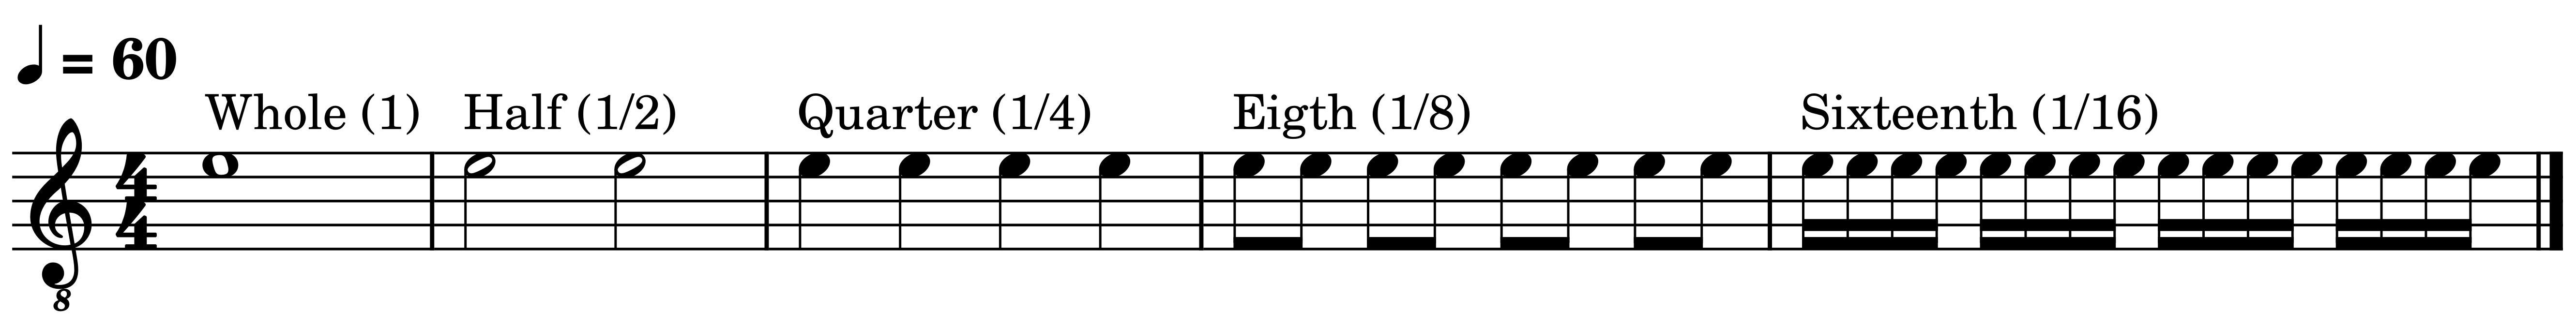
\includegraphics[width=\textwidth]{../../MuseScore/Guitar/MusicNotation/NoteDurations_Basic.png}
	\caption{Note duration}
	\label{fig:note_duration_basic}
\end{figure}

\textbf{Important}: A whole note (\wholeNote) equal 4 quarter notes (\quarterNote). It does \textbf{not} equal a whole measure. \newline

There are also other time signatures. But they all have the meaning. The top value indicated how many notes of the bottom number's duration fit in a measure. So a \lilyTimeSignature{3}{4} time signature can fit 3 quarter notes per measure. And a \lilyTimeSignature{6}{8} time signature can fit 6 eight notes per measure. Note that \lilyTimeSignature{3}{4} and \lilyTimeSignature{6}{8} actually indicate the same duration per measure, but they indicate a different feel. This is indicated in \ref{fig:time_signatures}

In \ref{fig:time_signatures} you also see a new duration notation. In the first measure with \lilyTimeSignature{6}{8} timing, there are dots next to the notes (\quarterNoteDottedDown). This means that the note has a duration of 1.5x its original duration.

The \lilyAccent symbol means that this note should be played with a more powerful accent. The bold numbers above the notes indicate the counting of the notes. A bold number means to put an accent on it, but played less accented then the ones where there is also an \lilyAccent symbol.

\begin{figure}[h]
	\centering
	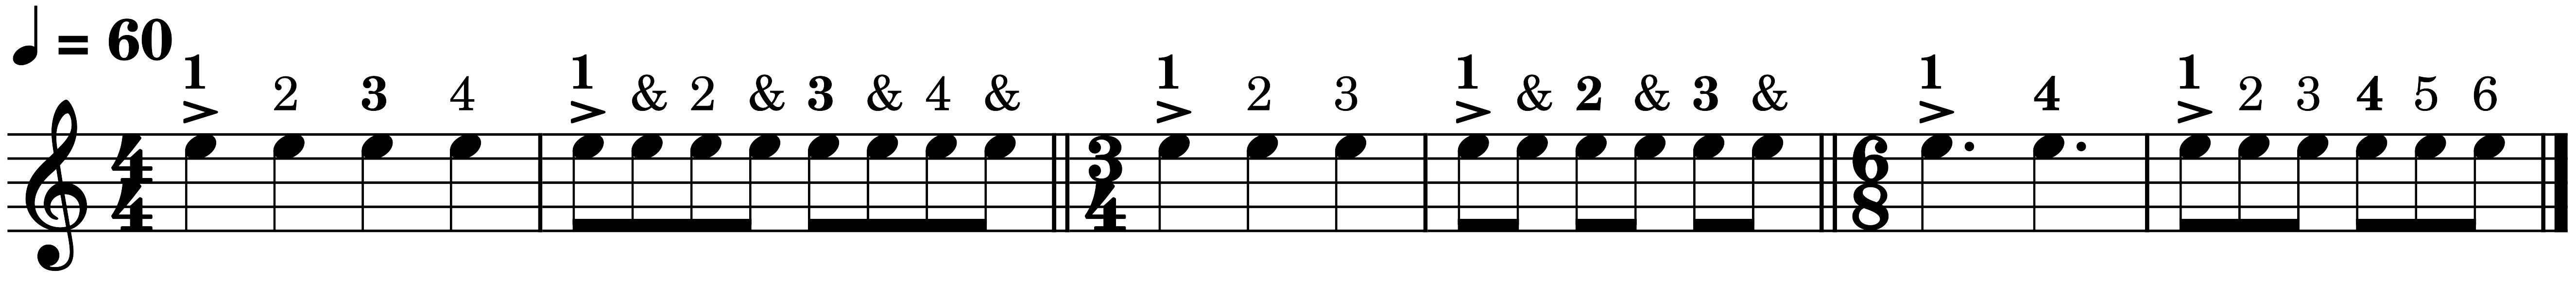
\includegraphics[width=\textwidth]{../../MuseScore/Guitar/MusicNotation/TimeSignature.png}
	\caption{Time signatures}
	\label{fig:time_signatures}
\end{figure}

Remember exercise \ref{fig:exercise_nothing_else_matters_metallica_intro_pima} (Metallica - Nothing else matters (intro))? That is also in \lilyTimeSignature{6}{8}.


\newpage

\subsection{Exercises}

As a first tune that uses multiple note durations, and to learn the first notes on the guitar, Jingle bells will be played (\ref{fig:jingle_bells}). The notes used for this tune are shown in \ref{fig:notes_in_jingle_bells}.

\begin{figure}[h]
	\centering
	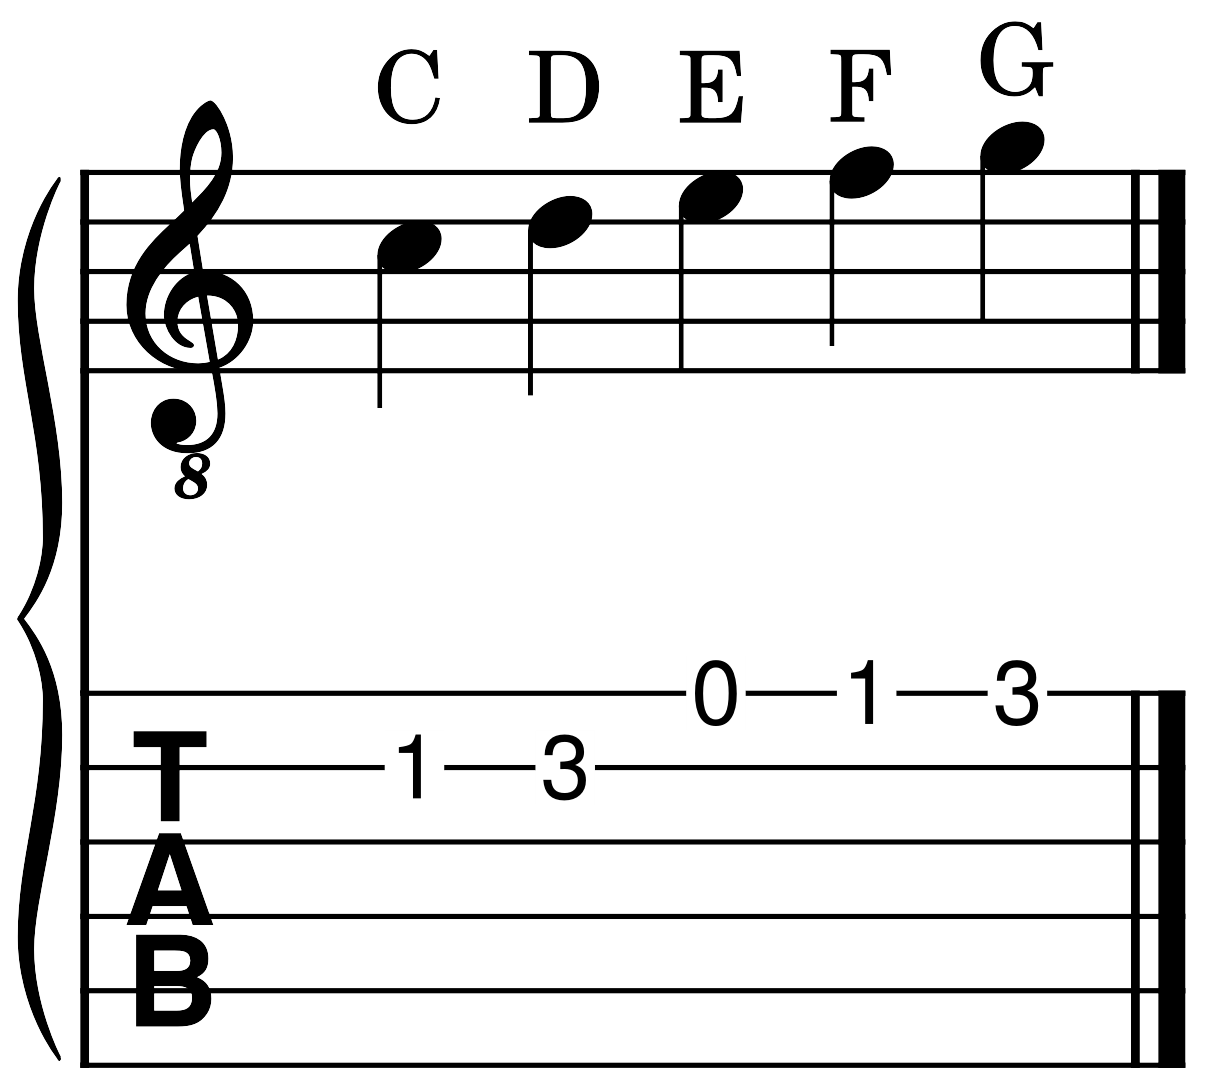
\includegraphics[height=0.12\textheight]{../../MuseScore/Guitar/NotesInJingleBells.png}
	\caption{Notes used in jingle bells}
	\label{fig:notes_in_jingle_bells}
\end{figure}

Now Jingle bells can be played as shown in \ref{fig:jingle_bells}.

\begin{figure}[h]
	\centering
	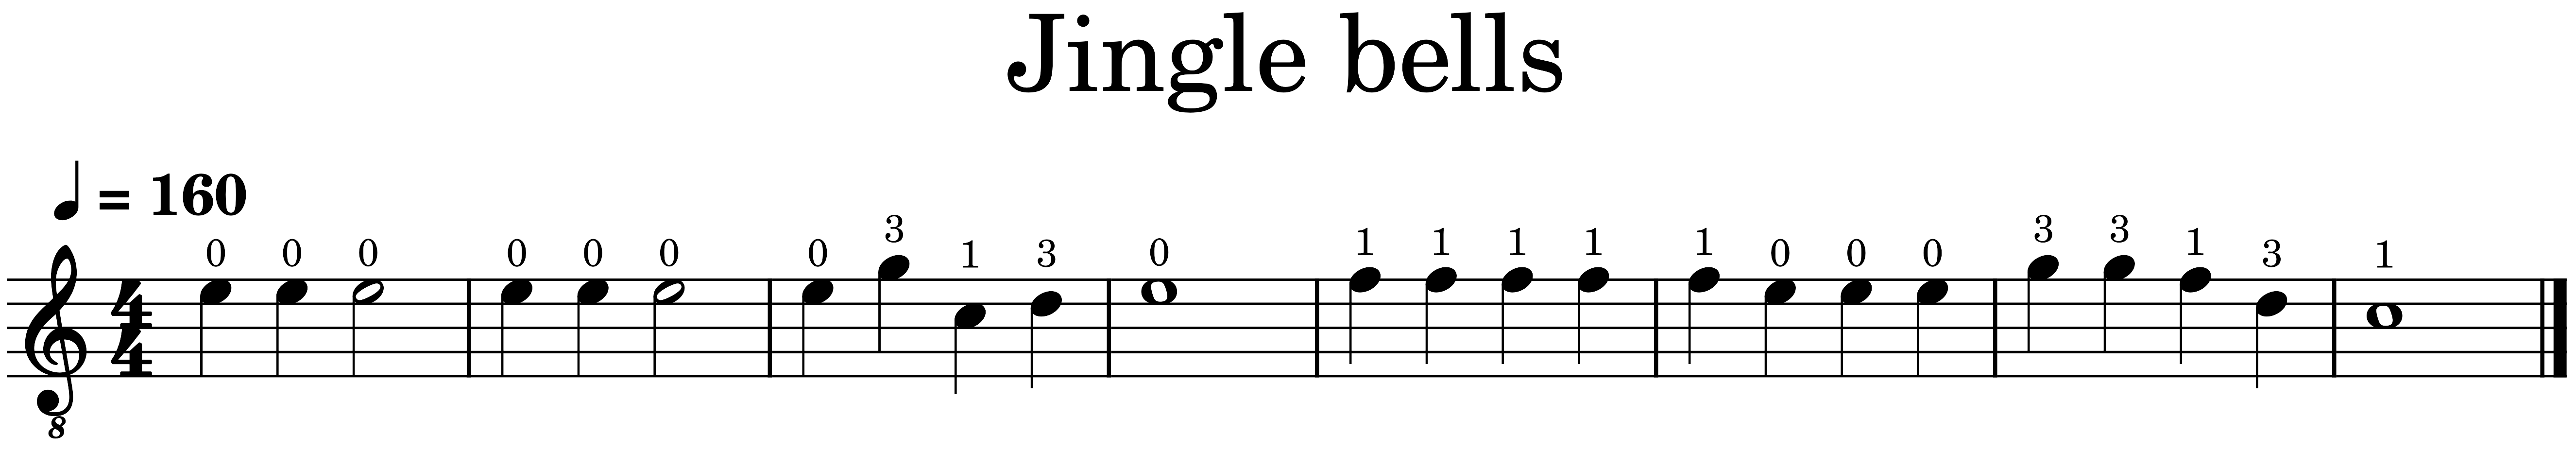
\includegraphics[width=\textwidth]{../../MuseScore/Guitar/JingleBells.png}
	\caption{Jingle bells}
	\label{fig:jingle_bells}
\end{figure}

\newpage

To learn a few more notes, the "Tetris" tune will be played. The notes from \ref{fig:notes_for_tetris_first_part} should are used in this tune. The only new notes are A and B.

\begin{figure}[h]
	\centering
	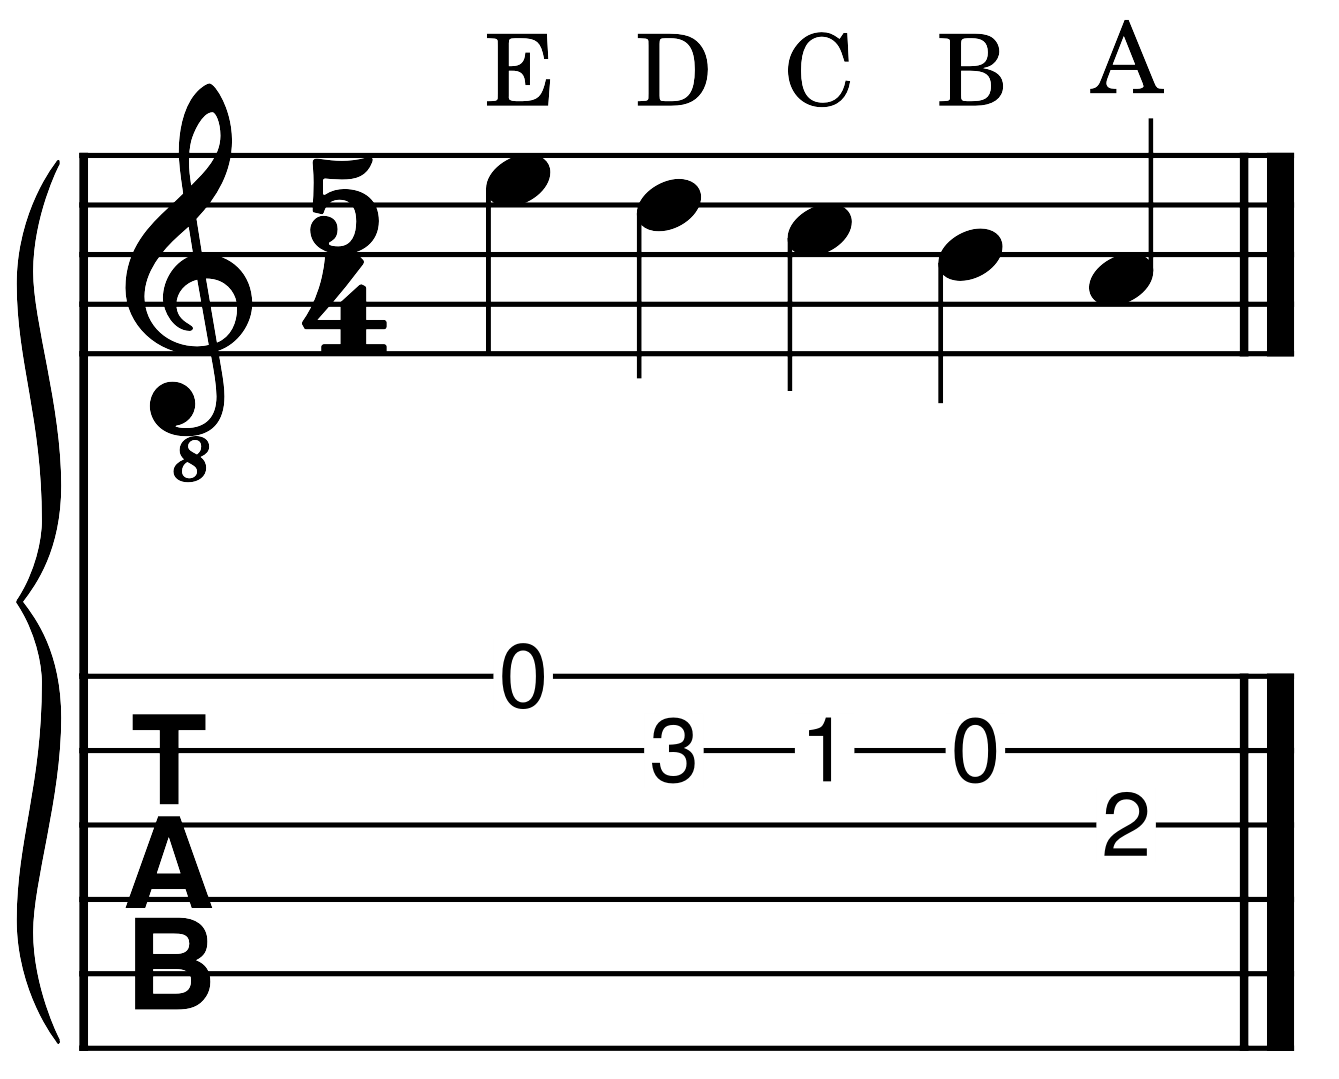
\includegraphics[height=0.12\textheight]{../../MuseScore/Guitar/NotesUsedInTetris_FirstPart.png}
	\caption{Notes used for the first part of the Tetris tune}
	\label{fig:notes_for_tetris_first_part}
\end{figure}

In \ref{fig:tetris_simple_first_part} the first part of the Tetris tune is written. Note the dotted note in measure 3.

\begin{figure}[h]
	\centering
	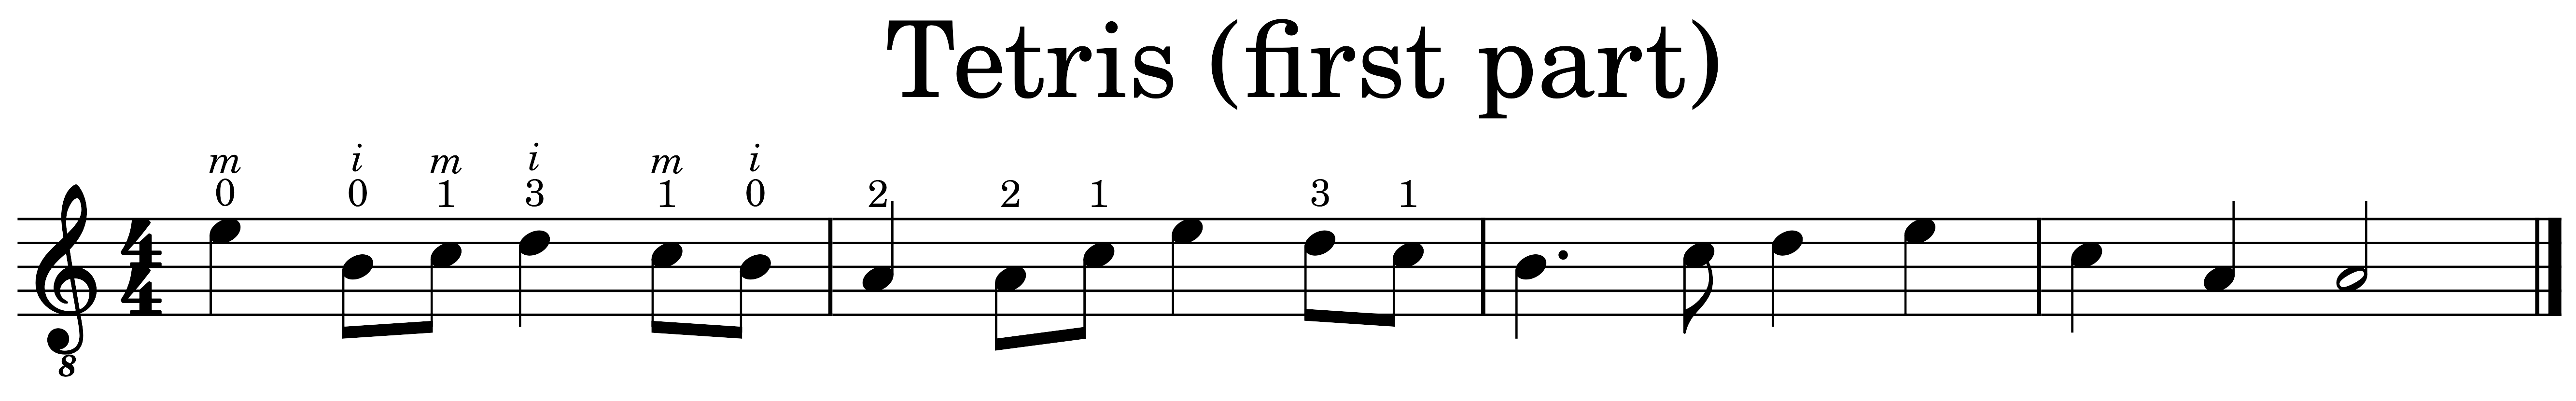
\includegraphics[width=\textwidth]{../../MuseScore/Guitar/Tetris_Simple_FirstPart.png}
	\caption{First part of the Tetris tune}
	\label{fig:tetris_simple_first_part}
\end{figure}


\infobox{The "Tetris" tune is actually derived from a Russian folk song called "Korobeiniki", which is based the a similar named poem written by Nikolai Nekrasov.}

\newpage

We have now played all non-sharp/flat notes. But each note can be placed in different positions, and with different pitches.

Let's take the melody of "Memory" from the musical "Cats" \ref{fig:memory_cats}. It uses most of the notes we already learned, but also uses a lower G, F, and E (\ref{fig:notes_g_f_e_3}).


\begin{figure}[h]
	\centering
	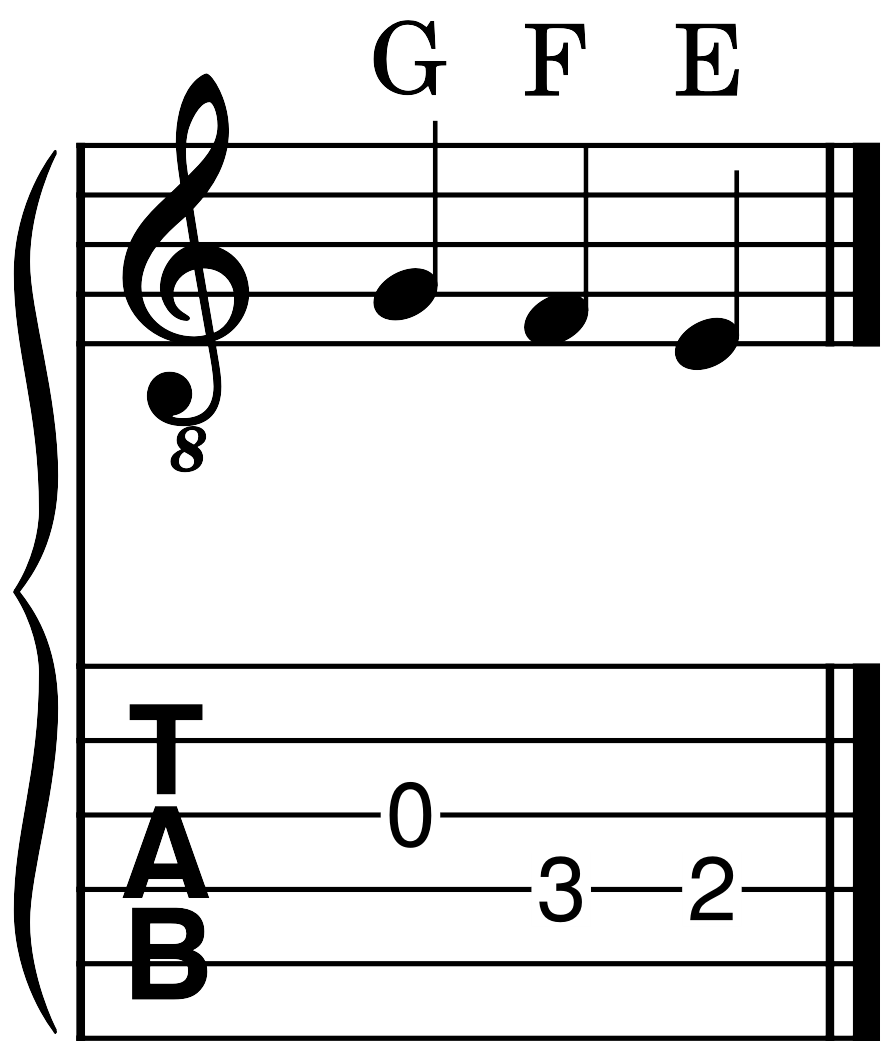
\includegraphics[height=0.12\textheight]{../../MuseScore/Guitar/NotesGFE3.png}
	\caption{The G, F, and G, notes on the 3rd and 4th strings}
	\label{fig:notes_g_f_e_3}
\end{figure}

It also uses a new symbol. The \textbf{tie} symbol (seen to connect notes from measure 5 and 6 in \ref{fig:memory_cats}). This symbol indicates that the duration of the first note that starts the tie has the summed duration of all consecutive identical note. All identical notes after the note that starts the tie are therefore not played

\begin{figure}[h]
	\centering
	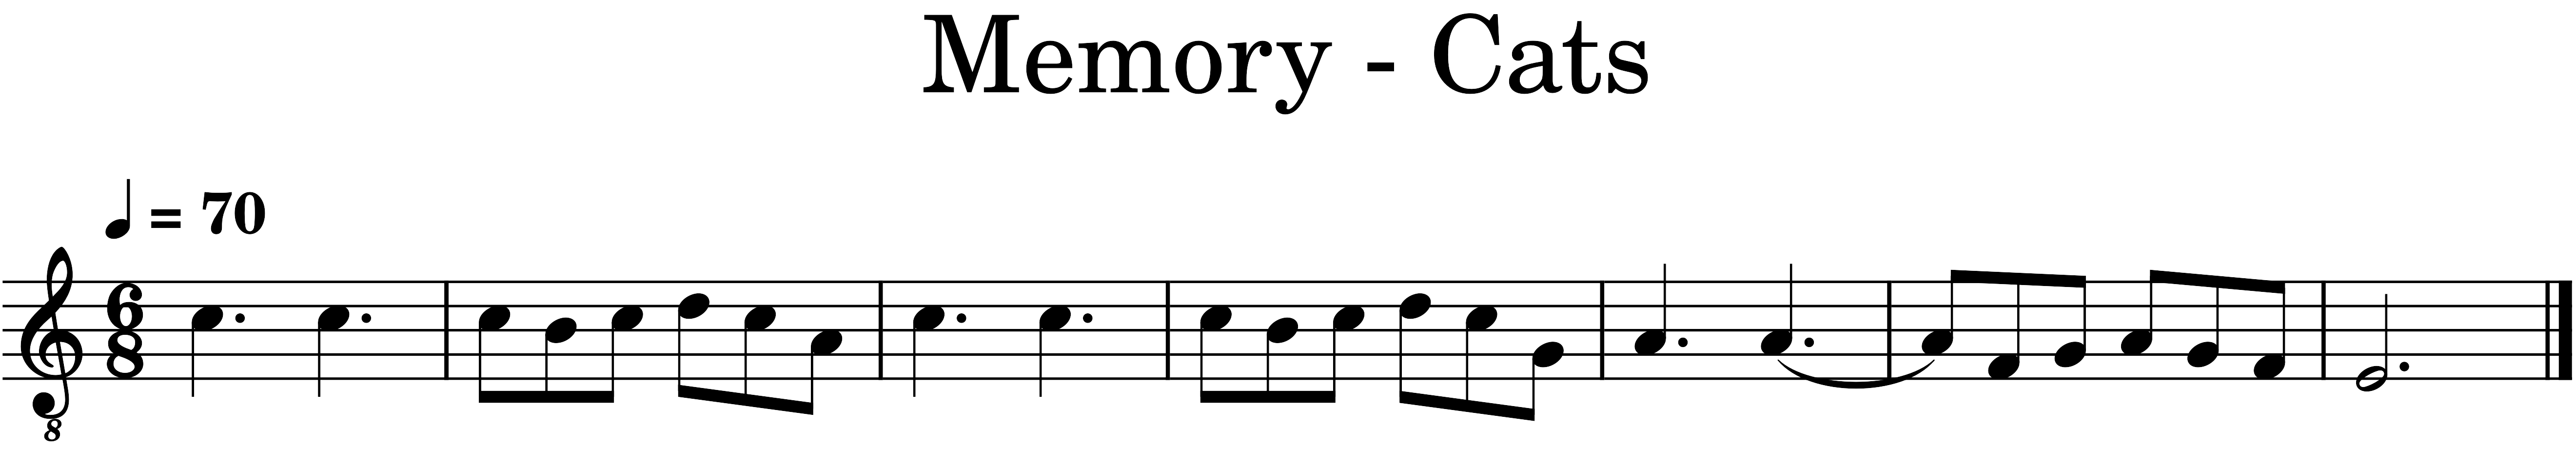
\includegraphics[width=\textwidth]{../../MuseScore/Guitar/MemoryCats.png}
	\caption{Memory from the musical Cats}
	\label{fig:memory_cats}
\end{figure}

\newpage

Another song that you know that uses all the notes that you've learned so far is Happy birthday {\ref{fig:happy_birthday}}. This notation also introduces a new symbol. The rest symbol \crotchetRest.

Just like there are multiple durations for notes, there are also multiple durations for rests. Before playing happy birthday, lets have a look at the different rest symbols in \ref{fig:rest_symbols}.

\begin{figure}[h]
	\centering
	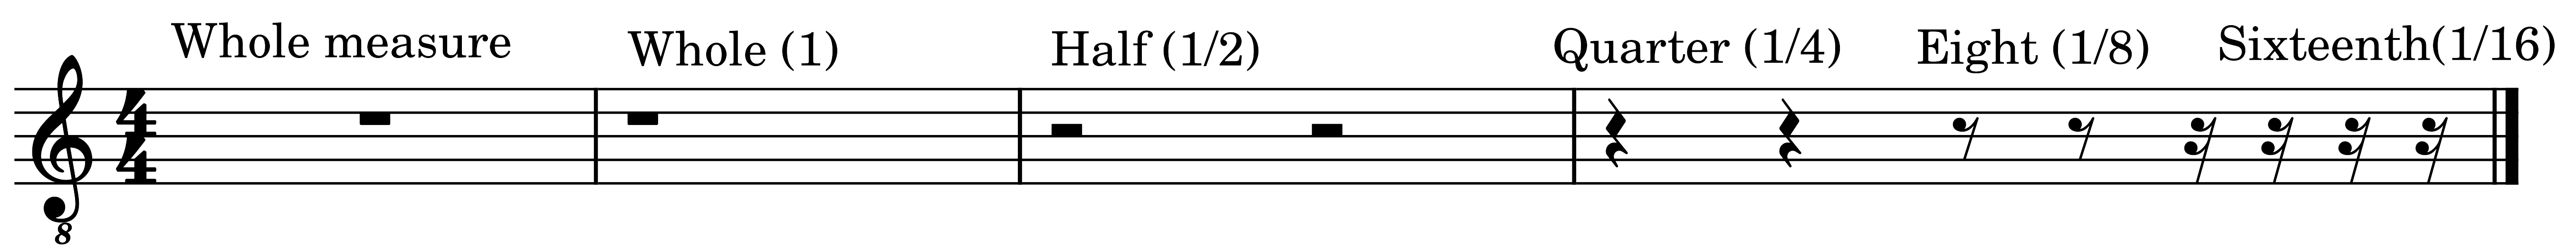
\includegraphics[width=\textwidth]{../../MuseScore/Guitar/Rests.png}
	\caption{Rest symbols}
	\label{fig:rest_symbols}
\end{figure}

\begin{figure}[h]
	\centering
	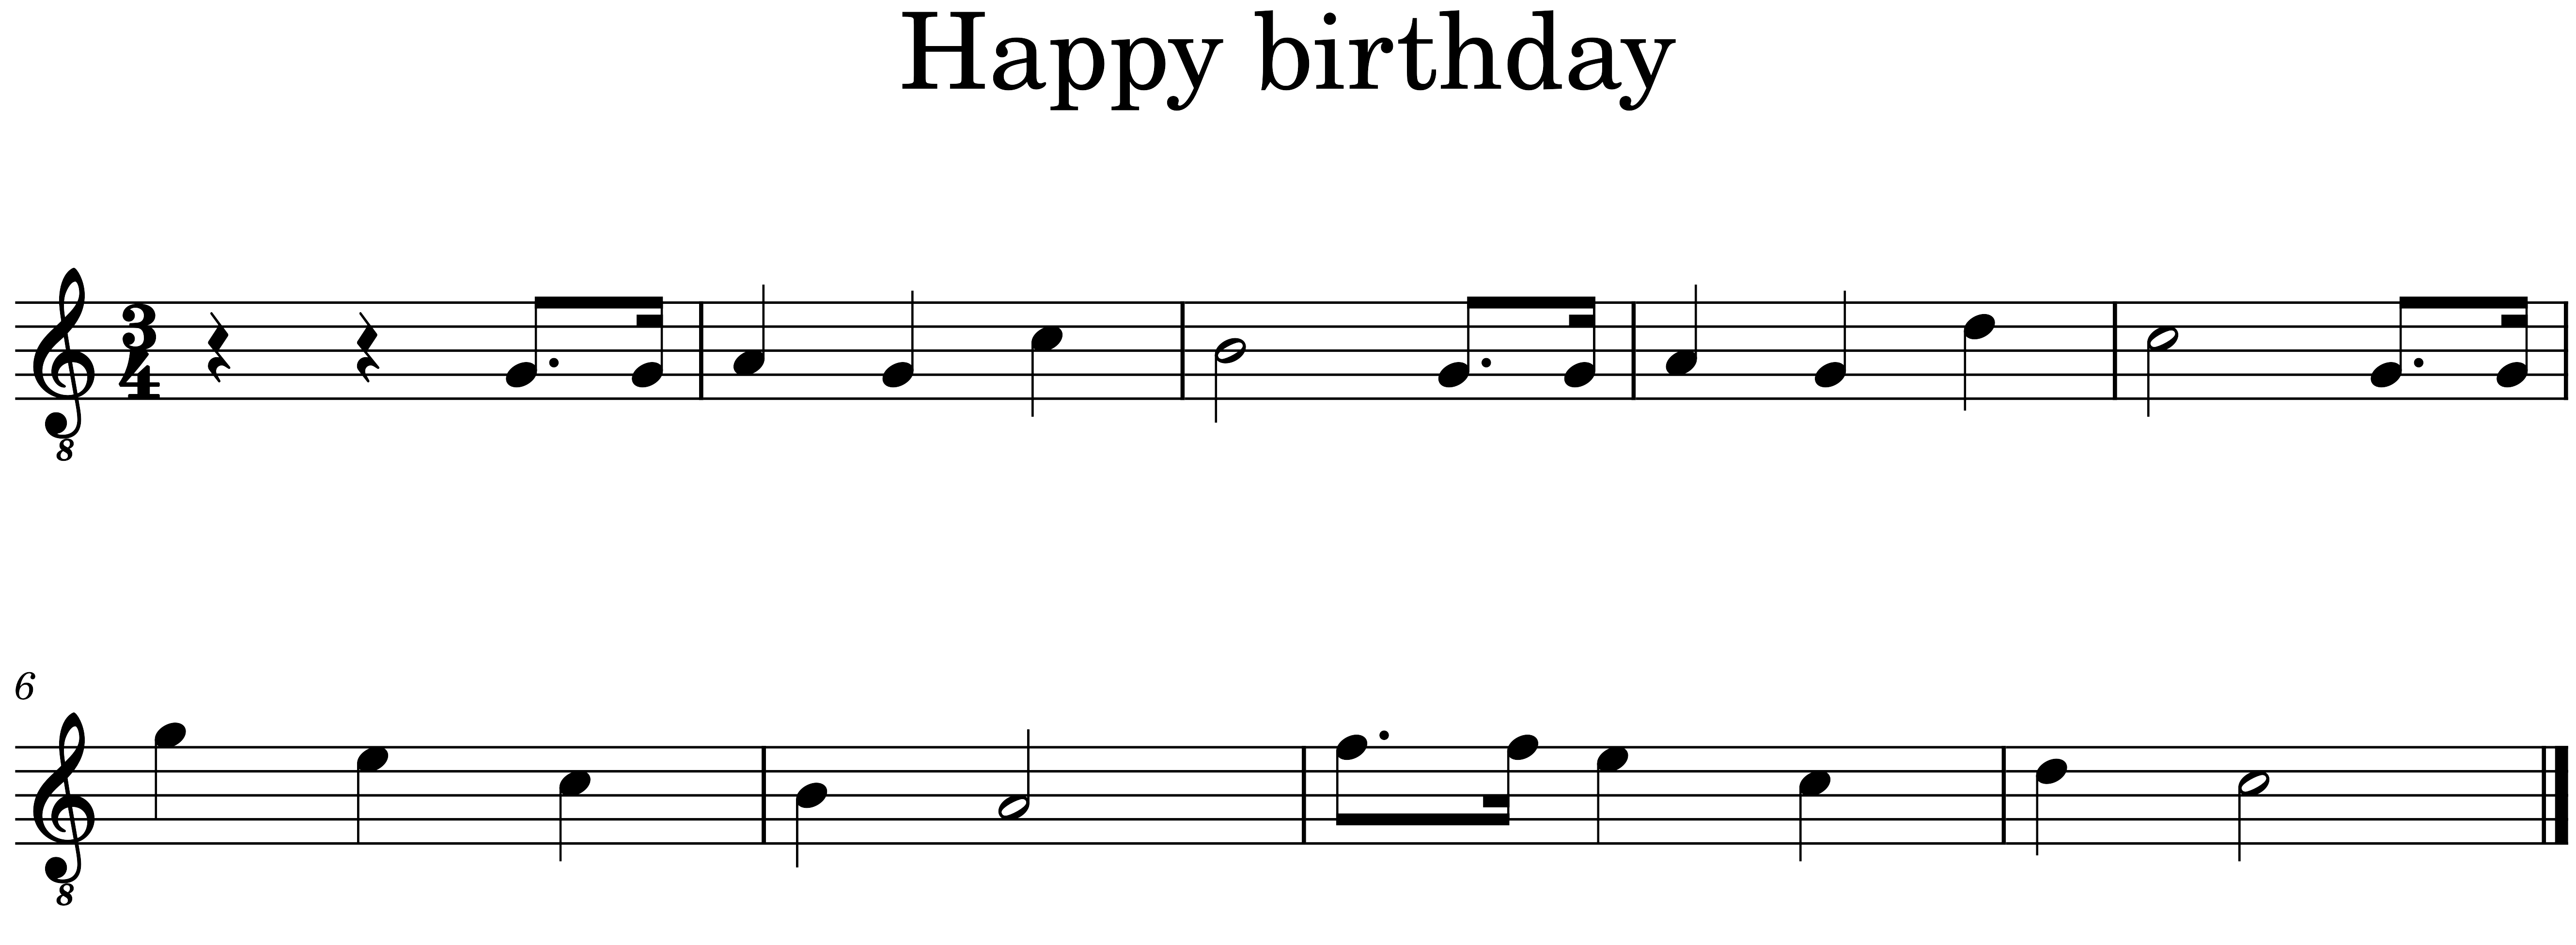
\includegraphics[width=\textwidth]{../../MuseScore/Guitar/HappyBirthday.png}
	\caption{Happy birthday}
	\label{fig:happy_birthday}
\end{figure}